\documentclass{subfiles}

\begin{document}

Uma \textit{Cadeia de Markov} é um processo estocástico no qual a probabilidade do próximo evento depende apenas do evento anterior. Neste trabalho focaremos apenas em modelos de tempo e estado discretos.

\begin{figure} % Single column figure
	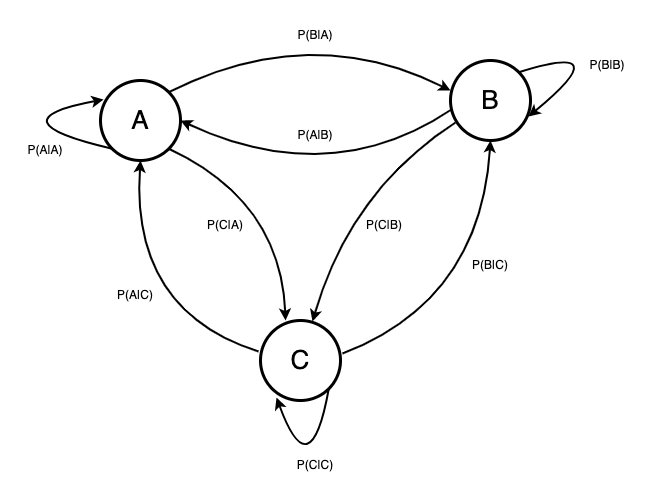
\includegraphics[width=\linewidth]{markov_chain.png}
	\caption{Diagrama de estados.}
	\label{fig:tcanther}
\end{figure}

por um conjunto de estados $E$, $\vert E \vert = n \in \mathbb{N}$ e uma matriz transição $T \in \mathbb{R}^{n \times n}$ que relaciona cada estado de partida a uma probabilidade para o estado de chegada. É, por tanto, uma representação de fenômenos em séries de tamanhos variados de forma discreta cuja a probabilidade do estado seguinte só depende do estado atual
\[
	P(E_{t_{i+1}} \vert E_{t_1}, \dots, E_{t_i}) = P(E_{t_{i+1}} \vert E_{t_i})
\]
Por exemplo, considere um processo que cria sequências aleatórias de letras
\begin{gather*}
	ABCABACCACAB         \\
	BACABACAAC           \\
	BBABAAAACCACABABABAC \\
\end{gather*}
Para recuperar os estados, observe que, há no total que 20 ocorrências da letra $A$, 11 de $B$, e 11 de $C$, calculando cada probabilidade
\begin{gather*}
	P(A|A) = 4/20 \\
	P(B|A) = 8/20 \\
	P(C|A) = 8/20 \\
	P(A|B) = 8/10 \\
	P(B|B) = 1/10 \\
	P(C|B) = 1/10 \\
	P(A|C) = 7/9  \\
	P(B|C) = 0/9  \\
	P(C|C) = 2/9
\end{gather*}
Por tanto, a estimativa da matriz transição que criou tais sequências é representado por
\[
	\begin{pmatrix}
		\frac{4}{20} & \frac{8}{20} & \frac{8}{20} \\
		\frac{8}{10} & \frac{1}{10} & \frac{1}{10} \\
		\frac{7}{9} & \frac{0}{9} & \frac{2}{9} \\
	\end{pmatrix}
\]
De posse desta matriz é possível descobrir o estado estacionário deste processo, ou seja, estimar a distribuição dos estados após quando a quantidade de observações vai ao infinito. Digamos 
Há também a possibilidade de expandir o modelo adicionando mais estados na dependência do estado seguinte, como Bishop\autocite{Bishop:2006pat} discute, mas isso vem com o custo de mais variáveis para se calcular. A medida que se adiciona $1$ estado na dependência, se multiplica a quantidade de parâmetros por $n$, a quantidade de estados. Este nível de detalhamento pode tornar o modelo impraticável quando esta expansão se torna muito grande.

\end{document}